\documentclass{article}

\usepackage{agda}


\usepackage{autofe}
\usepackage{amsmath,amsthm,thmtools,amssymb,amsfonts}
\declaretheorem[name=Theorem]{theorem}
\declaretheorem[name=Lemma]{lemma}

\DeclareUnicodeCharacter{10239}{\ensuremath{\rightsquigarrow}}
\DeclareUnicodeCharacter{8345}{\ensuremath{_n}}
\DeclareUnicodeCharacter{8902}{\ensuremath{^*\!}}
%\usepackage[language=english,eprint=false,doi=false]{biblatex}
%\addbibresource[location=remote]{http://www.citeulike.org/bibtex/user/miguelpagano/library?fieldmap=posted-at:posted-date&clean_urls=0}

\usepackage{tikz}
\usetikzlibrary{arrows}%,decorations.pathmorphing}

\usepackage{subfig}
%\title{A formalisation of Church-Rosser using parallel reductions}

\newcommand{\pred}{\Rightarrow}
\newcommand{\reduction}{\rightarrow}
\newcommand{\reduces}[2]{#1\,\rightarrow\,#2}
\newcommand{\reducesn}[2]{#1\,\rightarrow^{n}\,#2}
\newcommand{\transclos}[1]{#1^\ast}

%\maketitle

%% ODER: format ==         = "\mathrel{==}"
%% ODER: format /=         = "\neq "
%
%
\makeatletter
\@ifundefined{lhs2tex.lhs2tex.sty.read}%
  {\@namedef{lhs2tex.lhs2tex.sty.read}{}%
   \newcommand\SkipToFmtEnd{}%
   \newcommand\EndFmtInput{}%
   \long\def\SkipToFmtEnd#1\EndFmtInput{}%
  }\SkipToFmtEnd

\newcommand\ReadOnlyOnce[1]{\@ifundefined{#1}{\@namedef{#1}{}}\SkipToFmtEnd}
\usepackage{amstext}
\usepackage{amssymb}
\usepackage{stmaryrd}
\DeclareFontFamily{OT1}{cmtex}{}
\DeclareFontShape{OT1}{cmtex}{m}{n}
  {<5><6><7><8>cmtex8
   <9>cmtex9
   <10><10.95><12><14.4><17.28><20.74><24.88>cmtex10}{}
\DeclareFontShape{OT1}{cmtex}{m}{it}
  {<-> ssub * cmtt/m/it}{}
\newcommand{\texfamily}{\fontfamily{cmtex}\selectfont}
\DeclareFontShape{OT1}{cmtt}{bx}{n}
  {<5><6><7><8>cmtt8
   <9>cmbtt9
   <10><10.95><12><14.4><17.28><20.74><24.88>cmbtt10}{}
\DeclareFontShape{OT1}{cmtex}{bx}{n}
  {<-> ssub * cmtt/bx/n}{}
\newcommand{\tex}[1]{\text{\texfamily#1}}	% NEU

\newcommand{\Sp}{\hskip.33334em\relax}


\newcommand{\Conid}[1]{\mathit{#1}}
\newcommand{\Varid}[1]{\mathit{#1}}
\newcommand{\anonymous}{\kern0.06em \vbox{\hrule\@width.5em}}
\newcommand{\plus}{\mathbin{+\!\!\!+}}
\newcommand{\bind}{\mathbin{>\!\!\!>\mkern-6.7mu=}}
\newcommand{\rbind}{\mathbin{=\mkern-6.7mu<\!\!\!<}}% suggested by Neil Mitchell
\newcommand{\sequ}{\mathbin{>\!\!\!>}}
\renewcommand{\leq}{\leqslant}
\renewcommand{\geq}{\geqslant}
\usepackage{polytable}

%mathindent has to be defined
\@ifundefined{mathindent}%
  {\newdimen\mathindent\mathindent\leftmargini}%
  {}%

\def\resethooks{%
  \global\let\SaveRestoreHook\empty
  \global\let\ColumnHook\empty}
\newcommand*{\savecolumns}[1][default]%
  {\g@addto@macro\SaveRestoreHook{\savecolumns[#1]}}
\newcommand*{\restorecolumns}[1][default]%
  {\g@addto@macro\SaveRestoreHook{\restorecolumns[#1]}}
\newcommand*{\aligncolumn}[2]%
  {\g@addto@macro\ColumnHook{\column{#1}{#2}}}

\resethooks

\newcommand{\onelinecommentchars}{\quad-{}- }
\newcommand{\commentbeginchars}{\enskip\{-}
\newcommand{\commentendchars}{-\}\enskip}

\newcommand{\visiblecomments}{%
  \let\onelinecomment=\onelinecommentchars
  \let\commentbegin=\commentbeginchars
  \let\commentend=\commentendchars}

\newcommand{\invisiblecomments}{%
  \let\onelinecomment=\empty
  \let\commentbegin=\empty
  \let\commentend=\empty}

\visiblecomments

\newlength{\blanklineskip}
\setlength{\blanklineskip}{0.66084ex}

\newcommand{\hsindent}[1]{\quad}% default is fixed indentation
\let\hspre\empty
\let\hspost\empty
\newcommand{\NB}{\textbf{NB}}
\newcommand{\Todo}[1]{$\langle$\textbf{To do:}~#1$\rangle$}

\EndFmtInput
\makeatother
%
\long\def\ignore#1{}

\begin{document}

\section{Reflexive and Transitve Clousure of a Relation}

\ignore{
\begingroup\par\noindent\advance\leftskip\mathindent\(
\begin{pboxed}\SaveRestoreHook
\column{B}{@{}>{\hspre}l<{\hspost}@{}}%
\column{3}{@{}>{\hspre}l<{\hspost}@{}}%
\column{E}{@{}>{\hspre}l<{\hspost}@{}}%
\>[B]{}\mathbf{open}\;\mathbf{import}\;\Conid{Level}\;\mathbf{hiding}\;(\Varid{zero}){}\<[E]%
\\
\>[B]{}\mathbf{module}\;\Conid{Relation}\;\{\mskip1.5mu \Varid{l}\;\mathbin{:}\;\Conid{Level}\mskip1.5mu\}\;(\Conid{A}\;\mathbin{:}\;\Conid{Set}\;\Varid{l})\;\mathbf{where}{}\<[E]%
\\
\>[B]{}\hsindent{3}{}\<[3]%
\>[3]{}\mathbf{open}\;\mathbf{import}\;\Conid{Relation.Nullary}{}\<[E]%
\\
\>[B]{}\hsindent{3}{}\<[3]%
\>[3]{}\mathbf{import}\;\Conid{Relation.Binary}\;\Varid{as}\;\Conid{RB}{}\<[E]%
\\
\>[B]{}\hsindent{3}{}\<[3]%
\>[3]{}\mathbf{open}\;\mathbf{import}\;\Conid{Data.Product}{}\<[E]%
\ColumnHook
\end{pboxed}
\)\par\noindent\endgroup\resethooks
}


\ignore{
-- A binary relation over a set $A$ can be formalised as a propositional
-- function from $A \times A$, the next definition is the currified form.
-- A relation is reflexive if each element is related to itself, and it
-- is transitive whenever $a$ related to $b$ and $b$ related to $c$ implies
-- $a$ related to $c$.
}

\ignore{
\begingroup\par\noindent\advance\leftskip\mathindent\(
\begin{pboxed}\SaveRestoreHook
\column{B}{@{}>{\hspre}l<{\hspost}@{}}%
\column{3}{@{}>{\hspre}l<{\hspost}@{}}%
\column{E}{@{}>{\hspre}l<{\hspost}@{}}%
\>[3]{}\Conid{Rel}\;\mathbin{:}\;\Conid{Set}\;(\Varid{suc}\;\Varid{l}){}\<[E]%
\\
\>[3]{}\Conid{Rel}\;\mathrel{=}\;\Conid{RB.Rel}\;\Conid{A}\;\Varid{l}{}\<[E]%
\ColumnHook
\end{pboxed}
\)\par\noindent\endgroup\resethooks


The dual $R^{\mathit{op}}$ of a relation $R$ is defined by swapping the pairs.

\begingroup\par\noindent\advance\leftskip\mathindent\(
\begin{pboxed}\SaveRestoreHook
\column{B}{@{}>{\hspre}l<{\hspost}@{}}%
\column{3}{@{}>{\hspre}l<{\hspost}@{}}%
\column{E}{@{}>{\hspre}l<{\hspost}@{}}%
\>[3]{}\Varid{dual}\;\mathbin{:}\;\Conid{Rel}\;\Varid{→}\;\Conid{Rel}{}\<[E]%
\\
\>[3]{}\Varid{dual}\;\Conid{R}\;\Varid{m}\;\Varid{n}\;\mathrel{=}\;\Conid{R}\;\Varid{n}\;\Varid{m}{}\<[E]%
\ColumnHook
\end{pboxed}
\)\par\noindent\endgroup\resethooks

Given two relations $R$ and $S$ over $A$ we can take their union.

\begingroup\par\noindent\advance\leftskip\mathindent\(
\begin{pboxed}\SaveRestoreHook
\column{B}{@{}>{\hspre}l<{\hspost}@{}}%
\column{3}{@{}>{\hspre}l<{\hspost}@{}}%
\column{5}{@{}>{\hspre}l<{\hspost}@{}}%
\column{11}{@{}>{\hspre}l<{\hspost}@{}}%
\column{E}{@{}>{\hspre}l<{\hspost}@{}}%
\>[3]{}\mathbf{data}\;\Varid{\char95 ∪\char95 }\;(\Conid{R}\;\Conid{S}\;\mathbin{:}\;\Conid{Rel})\;\mathbin{:}\;\Conid{Rel}\;\mathbf{where}{}\<[E]%
\\
\>[3]{}\hsindent{2}{}\<[5]%
\>[5]{}\Varid{left}\;{}\<[11]%
\>[11]{}\mathbin{:}\;\Varid{∀}\;\{\mskip1.5mu \Varid{a}\;\Varid{b}\mskip1.5mu\}\;\Varid{→}\;\Conid{R}\;\Varid{a}\;\Varid{b}\;\Varid{→}\;(\Conid{R}\;\Varid{∪}\;\Conid{S})\;\Varid{a}\;\Varid{b}{}\<[E]%
\\
\>[3]{}\hsindent{2}{}\<[5]%
\>[5]{}\Varid{right}\;\mathbin{:}\;\Varid{∀}\;\{\mskip1.5mu \Varid{a}\;\Varid{b}\mskip1.5mu\}\;\Varid{→}\;\Conid{S}\;\Varid{a}\;\Varid{b}\;\Varid{→}\;(\Conid{R}\;\Varid{∪}\;\Conid{S})\;\Varid{a}\;\Varid{b}{}\<[E]%
\ColumnHook
\end{pboxed}
\)\par\noindent\endgroup\resethooks


Binary relations can be pre-ordered by inclusion, $R$ is less than or
equal to $S$ when $a\,R\,b$ implies $a\,S\,b$; as usual we write $R
\subseteq S$. 

\begingroup\par\noindent\advance\leftskip\mathindent\(
\begin{pboxed}\SaveRestoreHook
\column{B}{@{}>{\hspre}l<{\hspost}@{}}%
\column{3}{@{}>{\hspre}l<{\hspost}@{}}%
\column{E}{@{}>{\hspre}l<{\hspost}@{}}%
\>[3]{}\Varid{\char95 ⊆\char95 }\;\mathbin{:}\;\Conid{Rel}\;\Varid{→}\;\Conid{Rel}\;\Varid{→}\;\Conid{Set}\;\Varid{l}{}\<[E]%
\\
\>[3]{}\Conid{R}\;\Varid{⊆}\;\Conid{S}\;\mathrel{=}\;\Conid{RB.\char95 ⇒\char95 }\;\Conid{R}\;\Conid{S}{}\<[E]%
\\[\blanklineskip]%
\>[3]{}\Varid{refl-⊆}\;\mathbin{:}\;\{\mskip1.5mu \Conid{R}\;\mathbin{:}\;\Conid{Rel}\mskip1.5mu\}\;\Varid{→}\;\Conid{R}\;\Varid{⊆}\;\Conid{R}{}\<[E]%
\\
\>[3]{}\Varid{refl-⊆}\;\Varid{aRb}\;\mathrel{=}\;\Varid{aRb}{}\<[E]%
\\[\blanklineskip]%
\>[3]{}\Varid{trans-⊆}\;\mathbin{:}\;\{\mskip1.5mu \Conid{R}\;\Conid{S}\;\Conid{T}\;\mathbin{:}\;\Conid{Rel}\mskip1.5mu\}\;\Varid{→}\;\Conid{R}\;\Varid{⊆}\;\Conid{S}\;\Varid{→}\;\Conid{S}\;\Varid{⊆}\;\Conid{T}\;\Varid{→}\;\Conid{R}\;\Varid{⊆}\;\Conid{T}{}\<[E]%
\\
\>[3]{}\Varid{trans-⊆}\;\Conid{R⊆S}\;\Conid{S⊆T}\;\Varid{aRb}\;\mathrel{=}\;\Conid{S⊆T}\;(\Conid{R⊆S}\;\Varid{aRb}){}\<[E]%
\ColumnHook
\end{pboxed}
\)\par\noindent\endgroup\resethooks
}

The reflexive and transitive closure of a relation is more naturally
introduced by allowing more than one steps in the transitive clause.
Some immediate facts about the transitive closure of an operation is
that it is monotone and idempotent (besides these two properties one
asks that the closure of $R$ contains $R$, but this is immediate from
the definition). From these two properties we prove that $R \subseteq
\transclos S$ implies $\transclos R \subseteq \transclos S$
(alternatively one can proceed by induction on $a\,\transclos R\,b$); it is
straightforward to prove the other

\begingroup\par\noindent\advance\leftskip\mathindent\(
\begin{pboxed}\SaveRestoreHook
\column{B}{@{}>{\hspre}l<{\hspost}@{}}%
\column{3}{@{}>{\hspre}l<{\hspost}@{}}%
\column{5}{@{}>{\hspre}l<{\hspost}@{}}%
\column{12}{@{}>{\hspre}l<{\hspost}@{}}%
\column{16}{@{}>{\hspre}l<{\hspost}@{}}%
\column{E}{@{}>{\hspre}l<{\hspost}@{}}%
\>[3]{}\mathbf{data}\;\Varid{star}\;(\Varid{⟿}\;\mathbin{:}\;\Conid{Rel})\;\mathbin{:}\;\Conid{Rel}\;\mathbf{where}{}\<[E]%
\\
\>[3]{}\hsindent{2}{}\<[5]%
\>[5]{}\Varid{refl}\;\mathbin{:}\;\Varid{∀}\;\{\mskip1.5mu \Varid{a}\mskip1.5mu\}\;\Varid{→}\;\Varid{star}\;\Varid{⟿}\;\Varid{a}\;\Varid{a}{}\<[E]%
\\
\>[3]{}\hsindent{2}{}\<[5]%
\>[5]{}\Varid{just}\;\mathbin{:}\;\Varid{∀}\;\{\mskip1.5mu \Varid{a}\;\Varid{b}\mskip1.5mu\}\;\Varid{→}\;\Varid{⟿}\;\Varid{a}\;\Varid{b}\;\Varid{→}\;\Varid{star}\;\Varid{⟿}\;\Varid{a}\;\Varid{b}{}\<[E]%
\\
\>[3]{}\hsindent{2}{}\<[5]%
\>[5]{}\Varid{trans}\;\mathbin{:}\;\Varid{∀}\;\{\mskip1.5mu \Varid{a}\;\Varid{b}\;\Varid{c}\mskip1.5mu\}\;\Varid{→}\;\Varid{star}\;\Varid{⟿}\;\Varid{a}\;\Varid{b}\;\Varid{→}\;\Varid{star}\;\Varid{⟿}\;\Varid{b}\;\Varid{c}\;\Varid{→}\;\Varid{star}\;\Varid{⟿}\;\Varid{a}\;\Varid{c}{}\<[E]%
\\[\blanklineskip]%
\>[3]{}\mathbf{data}\;\Varid{equiv}\;(\Varid{⟿}\;\mathbin{:}\;\Conid{Rel})\;\mathbin{:}\;\Conid{Rel}\;\mathbf{where}{}\<[E]%
\\
\>[3]{}\hsindent{2}{}\<[5]%
\>[5]{}\Varid{≡-refl}\;\mathbin{:}\;\Varid{∀}\;\{\mskip1.5mu \Varid{a}\mskip1.5mu\}\;\Varid{→}\;\Varid{equiv}\;\Varid{⟿}\;\Varid{a}\;\Varid{a}{}\<[E]%
\\
\>[3]{}\hsindent{2}{}\<[5]%
\>[5]{}\Varid{≡-just}\;\mathbin{:}\;\Varid{∀}\;\{\mskip1.5mu \Varid{a}\;\Varid{b}\mskip1.5mu\}\;\Varid{→}\;\Varid{⟿}\;\Varid{a}\;\Varid{b}\;\Varid{→}\;\Varid{equiv}\;\Varid{⟿}\;\Varid{a}\;\Varid{b}{}\<[E]%
\\
\>[3]{}\hsindent{2}{}\<[5]%
\>[5]{}\Varid{≡-sym}\;{}\<[12]%
\>[12]{}\mathbin{:}\;\Varid{∀}\;\{\mskip1.5mu \Varid{a}\;\Varid{b}\mskip1.5mu\}\;\Varid{→}\;\Varid{equiv}\;\Varid{⟿}\;\Varid{a}\;\Varid{b}\;\Varid{→}\;\Varid{equiv}\;\Varid{⟿}\;\Varid{b}\;\Varid{a}{}\<[E]%
\\
\>[3]{}\hsindent{2}{}\<[5]%
\>[5]{}\Varid{≡-trans}\;\mathbin{:}\;\Varid{∀}\;\{\mskip1.5mu \Varid{a}\;\Varid{b}\;\Varid{c}\mskip1.5mu\}\;\Varid{→}\;\Varid{equiv}\;\Varid{⟿}\;\Varid{a}\;\Varid{b}\;\Varid{→}\;\Varid{equiv}\;\Varid{⟿}\;\Varid{b}\;\Varid{c}\;\Varid{→}\;\Varid{equiv}\;\Varid{⟿}\;\Varid{a}\;\Varid{c}{}\<[E]%
\\[\blanklineskip]%
\>[3]{}\Varid{mon-star}\;\mathbin{:}\;\{\mskip1.5mu \Conid{R}\;\Conid{S}\;\mathbin{:}\;\Conid{Rel}\mskip1.5mu\}\;\Varid{→}\;\Conid{R}\;\Varid{⊆}\;\Conid{S}\;\Varid{→}\;\Varid{star}\;\Conid{R}\;\Varid{⊆}\;\Varid{star}\;\Conid{S}{}\<[E]%
\\
\>[3]{}\Varid{mon-star}\;\Conid{R⊆S}\;\Varid{refl}\;\mathrel{=}\;\Varid{refl}{}\<[E]%
\\
\>[3]{}\Varid{mon-star}\;\Conid{R⊆S}\;(\Varid{just}\;\Varid{aRb})\;\mathrel{=}\;\Varid{just}\;(\Conid{R⊆S}\;\Varid{aRb}){}\<[E]%
\\
\>[3]{}\Varid{mon-star}\;\Conid{R⊆S}\;(\Varid{trans}\;\Varid{aR⋆b}\;\Varid{bR⋆c})\;{}\<[E]%
\\
\>[3]{}\hsindent{2}{}\<[5]%
\>[5]{}\mathrel{=}\;\Varid{trans}\;(\Varid{mon-star}\;\Conid{R⊆S}\;\Varid{aR⋆b})\;(\Varid{mon-star}\;\Conid{R⊆S}\;\Varid{bR⋆c}){}\<[E]%
\\[\blanklineskip]%
\>[3]{}\Varid{idem-star}\;\mathbin{:}\;\{\mskip1.5mu \Conid{R}\;\mathbin{:}\;\Conid{Rel}\mskip1.5mu\}\;\Varid{→}\;\Varid{star}\;(\Varid{star}\;\Conid{R})\;\Varid{⊆}\;\Varid{star}\;\Conid{R}{}\<[E]%
\\
\>[3]{}\Varid{idem-star}\;\Varid{refl}\;\mathrel{=}\;\Varid{refl}{}\<[E]%
\\
\>[3]{}\Varid{idem-star}\;(\Varid{just}\;\Varid{aRb})\;\mathrel{=}\;\Varid{aRb}{}\<[E]%
\\
\>[3]{}\Varid{idem-star}\;(\Varid{trans}\;\Varid{aR⋆b}\;\Varid{bR⋆c})\;\mathrel{=}\;\Varid{trans}\;(\Varid{idem-star}\;\Varid{aR⋆b})\;(\Varid{idem-star}\;\Varid{bR⋆c}){}\<[E]%
\\[\blanklineskip]%
\>[3]{}\Varid{trans-⊆-star}\;\mathbin{:}\;\{\mskip1.5mu \Conid{R}\;\Conid{S}\;\mathbin{:}\;\Conid{Rel}\mskip1.5mu\}\;\Varid{→}\;\Conid{R}\;\Varid{⊆}\;\Varid{star}\;\Conid{S}\;\Varid{→}\;\Varid{star}\;\Conid{R}\;\Varid{⊆}\;\Varid{star}\;\Conid{S}{}\<[E]%
\\
\>[3]{}\Varid{trans-⊆-star}\;\{\mskip1.5mu \Conid{R}\mskip1.5mu\}\;\{\mskip1.5mu \Conid{S}\mskip1.5mu\}\;\Conid{R⊆S⋆}\;{}\<[E]%
\\
\>[3]{}\hsindent{2}{}\<[5]%
\>[5]{}\mathrel{=}\;\Varid{trans-⊆}\;{}\<[16]%
\>[16]{}\{\mskip1.5mu \Varid{star}\;\Conid{R}\mskip1.5mu\}\;\{\mskip1.5mu \Varid{star}\;(\Varid{star}\;\Conid{S})\mskip1.5mu\}\;\{\mskip1.5mu \Varid{star}\;\Conid{S}\mskip1.5mu\}\;{}\<[E]%
\\
\>[16]{}(\Varid{mon-star}\;\Conid{R⊆S⋆})\;{}\<[E]%
\\
\>[16]{}\Varid{idem-star}{}\<[E]%
\ColumnHook
\end{pboxed}
\)\par\noindent\endgroup\resethooks

Our next goal is to prove that the diamond property implies
Church-Rosser; for this it turns out that dealing with the usual
definition of the reflexive transitive closure is not convenient,
because the termination checker is not convinced about the use of the
inductive hypothesis in one case. In order to bypass this obstacle we
present another formalisation of the reflexive and transitive closure
of a relation $R^\omega = \bigcup_{n\in \mathbb N} R^n$; although
these two notions are not isomorphic (when passing from $\transclos R$ to
$R^{\omega}$ we lane all the single steps to the left), they are
equivalent.

\begingroup\par\noindent\advance\leftskip\mathindent\(
\begin{pboxed}\SaveRestoreHook
\column{B}{@{}>{\hspre}l<{\hspost}@{}}%
\column{3}{@{}>{\hspre}l<{\hspost}@{}}%
\column{5}{@{}>{\hspre}l<{\hspost}@{}}%
\column{11}{@{}>{\hspre}l<{\hspost}@{}}%
\column{24}{@{}>{\hspre}l<{\hspost}@{}}%
\column{47}{@{}>{\hspre}l<{\hspost}@{}}%
\column{48}{@{}>{\hspre}l<{\hspost}@{}}%
\column{49}{@{}>{\hspre}l<{\hspost}@{}}%
\column{E}{@{}>{\hspre}l<{\hspost}@{}}%
\>[3]{}\mathbf{data}\;\Varid{steps}\;(\Varid{⟿}\;\mathbin{:}\;\Conid{Rel})\;\mathbin{:}\;\Conid{Rel}\;\mathbf{where}{}\<[E]%
\\
\>[3]{}\hsindent{2}{}\<[5]%
\>[5]{}\Varid{zero}\;{}\<[11]%
\>[11]{}\mathbin{:}\;\Varid{∀}\;\{\mskip1.5mu \Varid{a}\mskip1.5mu\}\;{}\<[49]%
\>[49]{}\Varid{→}\;\Varid{steps}\;\Varid{⟿}\;\Varid{a}\;\Varid{a}{}\<[E]%
\\
\>[3]{}\hsindent{2}{}\<[5]%
\>[5]{}\Varid{one}\;{}\<[11]%
\>[11]{}\mathbin{:}\;\Varid{∀}\;\{\mskip1.5mu \Varid{a}\;\Varid{b}\mskip1.5mu\}\;{}\<[24]%
\>[24]{}\Varid{→}\;\Varid{⟿}\;\Varid{a}\;\Varid{b}\;{}\<[48]%
\>[48]{}\Varid{→}\;\Varid{steps}\;\Varid{⟿}\;\Varid{a}\;\Varid{b}{}\<[E]%
\\
\>[3]{}\hsindent{2}{}\<[5]%
\>[5]{}\Varid{more}\;{}\<[11]%
\>[11]{}\mathbin{:}\;\Varid{∀}\;\{\mskip1.5mu \Varid{a}\;\Varid{b}\;\Varid{c}\mskip1.5mu\}\;{}\<[24]%
\>[24]{}\Varid{→}\;\Varid{⟿}\;\Varid{a}\;\Varid{b}\;\Varid{→}\;\Varid{steps}\;\Varid{⟿}\;\Varid{b}\;\Varid{c}\;{}\<[47]%
\>[47]{}\Varid{→}\;\Varid{steps}\;\Varid{⟿}\;\Varid{a}\;\Varid{c}{}\<[E]%
\\[\blanklineskip]%
\>[3]{}\Varid{\char95 ++\char95 }\;\mathbin{:}\;{}\<[11]%
\>[11]{}\{\mskip1.5mu \Varid{⟿}\;\mathbin{:}\;\Conid{Rel}\mskip1.5mu\}\;\{\mskip1.5mu \Varid{a}\;\Varid{b}\;\Varid{c}\;\mathbin{:}\;\Conid{A}\mskip1.5mu\}\;{}\<[E]%
\\
\>[11]{}\Varid{→}\;\Varid{steps}\;\Varid{⟿}\;\Varid{a}\;\Varid{b}\;\Varid{→}\;\Varid{steps}\;\Varid{⟿}\;\Varid{b}\;\Varid{c}\;\Varid{→}\;\Varid{steps}\;\Varid{⟿}\;\Varid{a}\;\Varid{c}{}\<[E]%
\\
\>[3]{}\Varid{zero}\;\plus \;\Varid{s'}\;\mathrel{=}\;\Varid{s'}{}\<[E]%
\\
\>[3]{}\Varid{one}\;\Varid{a⟿b}\;\plus \;\Varid{b⟿*c}\;\mathrel{=}\;\Varid{more}\;\Varid{a⟿b}\;\Varid{b⟿*c}{}\<[E]%
\\
\>[3]{}\Varid{more}\;\Varid{a⟿b}\;\Varid{b⟿*c}\;\plus \;\Varid{c⟿*d}\;\mathrel{=}\;\Varid{more}\;\Varid{a⟿b}\;(\Varid{b⟿*c}\;\plus \;\Varid{c⟿*d}){}\<[E]%
\\[\blanklineskip]%
\>[3]{}\Varid{⋆-to-ω}\;\mathbin{:}\;\Varid{∀}\;\{\mskip1.5mu \Varid{a}\;\Varid{b}\;\Varid{⟿}\mskip1.5mu\}\;\Varid{→}\;\Varid{star}\;\Varid{⟿}\;\Varid{a}\;\Varid{b}\;\Varid{→}\;\Varid{steps}\;\Varid{⟿}\;\Varid{a}\;\Varid{b}{}\<[E]%
\\
\>[3]{}\Varid{⋆-to-ω}\;\Varid{refl}\;\mathrel{=}\;\Varid{zero}{}\<[E]%
\\
\>[3]{}\Varid{⋆-to-ω}\;(\Varid{just}\;\Varid{a⟿b})\;\mathrel{=}\;\Varid{one}\;\Varid{a⟿b}{}\<[E]%
\\
\>[3]{}\Varid{⋆-to-ω}\;(\Varid{trans}\;\Varid{a⟿*b}\;\Varid{b⟿*c})\;\mathrel{=}\;\Varid{⋆-to-ω}\;\Varid{a⟿*b}\;\plus \;\Varid{⋆-to-ω}\;\Varid{b⟿*c}{}\<[E]%
\\[\blanklineskip]%
\>[3]{}\Varid{ω-to-⋆}\;\mathbin{:}\;\Varid{∀}\;\{\mskip1.5mu \Varid{a}\;\Varid{b}\;\Varid{⟿}\mskip1.5mu\}\;\Varid{→}\;\Varid{steps}\;\Varid{⟿}\;\Varid{a}\;\Varid{b}\;\Varid{→}\;\Varid{star}\;\Varid{⟿}\;\Varid{a}\;\Varid{b}{}\<[E]%
\\
\>[3]{}\Varid{ω-to-⋆}\;\Varid{zero}\;\mathrel{=}\;\Varid{refl}{}\<[E]%
\\
\>[3]{}\Varid{ω-to-⋆}\;(\Varid{one}\;\Varid{a⟿b})\;\mathrel{=}\;\Varid{just}\;\Varid{a⟿b}{}\<[E]%
\\
\>[3]{}\Varid{ω-to-⋆}\;(\Varid{more}\;\Varid{a⟿b}\;\Varid{b⟿*c})\;\mathrel{=}\;\Varid{trans}\;(\Varid{just}\;\Varid{a⟿b})\;(\Varid{ω-to-⋆}\;\Varid{b⟿*c}){}\<[E]%
\ColumnHook
\end{pboxed}
\)\par\noindent\endgroup\resethooks

A relation $R$ is said to have the \emph{diamond} property if whenever
$a\,R\,b$ and $a\,R\,c$, there is a $d$ such that $b\,R\,d$ and
$c\,R\,d$; we will say that $R$ is \emph{diamantine} if it satisfies
the diamond property.

\begin{minipage}{0.7\textwidth}
\begingroup\par\noindent\advance\leftskip\mathindent\(
\begin{pboxed}\SaveRestoreHook
\column{B}{@{}>{\hspre}l<{\hspost}@{}}%
\column{3}{@{}>{\hspre}l<{\hspost}@{}}%
\column{18}{@{}>{\hspre}l<{\hspost}@{}}%
\column{19}{@{}>{\hspre}l<{\hspost}@{}}%
\column{E}{@{}>{\hspre}l<{\hspost}@{}}%
\>[3]{}\Varid{diamond}\;\mathbin{:}\;(\Varid{\char95 ⟿\char95 }\;\mathbin{:}\;\Conid{Rel})\;\Varid{→}\;\Conid{Set}\;\Varid{l}{}\<[E]%
\\
\>[3]{}\Varid{diamond}\;\Varid{\char95 ⟿\char95 }\;\mathrel{=}\;{}\<[18]%
\>[18]{}\{\mskip1.5mu \Varid{a}\;\Varid{b}\;\Varid{c}\;\mathbin{:}\;\Conid{A}\mskip1.5mu\}\;{}\<[E]%
\\
\>[18]{}\hsindent{1}{}\<[19]%
\>[19]{}\Varid{→}\;\Varid{a}\;\Varid{⟿}\;\Varid{b}\;\Varid{→}\;\Varid{a}\;\Varid{⟿}\;\Varid{c}\;\Varid{→}\;{}\<[E]%
\\
\>[18]{}\hsindent{1}{}\<[19]%
\>[19]{}\Varid{∃}\;(\Varid{λ}\;\Varid{d}\;\Varid{→}\;\Varid{b}\;\Varid{⟿}\;\Varid{d}\;\Varid{×}\;\Varid{c}\;\Varid{⟿}\;\Varid{d}){}\<[E]%
\ColumnHook
\end{pboxed}
\)\par\noindent\endgroup\resethooks
\end{minipage}
\begin{minipage}{0.3\textwidth}
\begin{tikzpicture}[>=latex]
   \node (a) at (2,2) {$a$};
   \node (b) at (1,1) {$b$};
   \node (c) at (3,1) {$c$};
   \node (d) at (2,0) {$d$};

   \draw [->] (a) -- (b) ;
   \draw [->] (a) -- (c) ;
   \draw[dashed,->] (b) -- (d) ;
   \draw[dashed,->] (c) -> (d) ;
\end{tikzpicture}
\end{minipage}

A relation $R$ is \emph{Church-Rosser} if its transitive closure is
diamantine; as we have already mentioned it is easier to deal with the
statement of Church-Rosser for the $n$-fold version of the transitive
closure.

\begingroup\par\noindent\advance\leftskip\mathindent\(
\begin{pboxed}\SaveRestoreHook
\column{B}{@{}>{\hspre}l<{\hspost}@{}}%
\column{3}{@{}>{\hspre}l<{\hspost}@{}}%
\column{5}{@{}>{\hspre}l<{\hspost}@{}}%
\column{E}{@{}>{\hspre}l<{\hspost}@{}}%
\>[3]{}\Varid{cr}\;\mathbin{:}\;(\Varid{⟿}\;\mathbin{:}\;\Conid{Rel})\;\Varid{→}\;\Conid{Set}\;\Varid{l}{}\<[E]%
\\
\>[3]{}\Varid{cr}\;\Varid{⟿}\;\mathrel{=}\;\Varid{diamond}\;(\Varid{star}\;\Varid{⟿}){}\<[E]%
\\[\blanklineskip]%
\>[3]{}\Varid{cr-steps}\;\mathbin{:}\;(\Varid{⟿}\;\mathbin{:}\;\Conid{Rel})\;\Varid{→}\;\Conid{Set}\;\Varid{l}{}\<[E]%
\\
\>[3]{}\Varid{cr-steps}\;\Varid{⟿}\;\mathrel{=}\;\Varid{diamond}\;(\Varid{steps}\;\Varid{⟿}){}\<[E]%
\\[\blanklineskip]%
\>[3]{}\Varid{cr-steps-to-cr}\;\mathbin{:}\;\{\mskip1.5mu \Varid{⟿}\;\mathbin{:}\;\Conid{Rel}\mskip1.5mu\}\;\Varid{→}\;\Varid{cr-steps}\;\Varid{⟿}\;\Varid{→}\;\Varid{cr}\;\Varid{⟿}{}\<[E]%
\\
\>[3]{}\Varid{cr-steps-to-cr}\;\Varid{cr}\;\Varid{a⟿*b}\;\Varid{a⟿*c}{}\<[E]%
\\
\>[3]{}\hsindent{2}{}\<[5]%
\>[5]{}\mathbf{with}\;\Varid{cr}\;(\Varid{⋆-to-ω}\;\Varid{a⟿*b})\;(\Varid{⋆-to-ω}\;\Varid{a⟿*c}){}\<[E]%
\\
\>[3]{}\Varid{...}\;\mid \;\Varid{d},\Varid{b⟿*d},\Varid{c⟿*d}\;\mathrel{=}\;\Varid{d},\Varid{ω-to-⋆}\;\Varid{b⟿*d},\Varid{ω-to-⋆}\;\Varid{c⟿*d}{}\<[E]%
\ColumnHook
\end{pboxed}
\)\par\noindent\endgroup\resethooks

\begin{lemma}
Let $\reduction$ have the diamond property; if there is a reduction
$\reduces a b$ and also a reduction $\reducesn a c$, then there exists
$d$ such that $\reducesn b d$ and $\reduces c d$.
\end{lemma}
\begin{proof}
The proof is by induction in the length of $\reduces a c$:

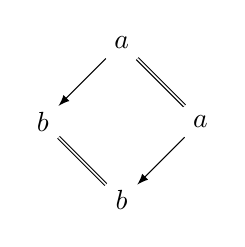
\begin{tikzpicture}[>=latex,baseline]
   \node (a) at (2,2) {$a$};
   \node (b) at (1,1) {$b$};
   \node (c) at (3,1) {$a$};
   \node (d) at (2,0) {$b$};

   \draw [->] (a) -- (b) ;
   \draw [double] (a) -- (c) ;
   \draw [double] (b) -- (d) ;
   \draw[->] (c) -> (d) ;
\end{tikzpicture} 
\quad
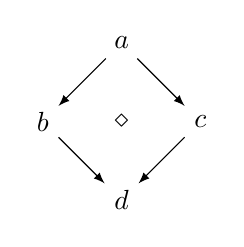
\begin{tikzpicture}[>=latex,baseline]
   \node (a) at (2,2) {$a$};
   \node (b) at (1,1) {$b$};
   \node (c) at (3,1) {$c$};
   \node (d) at (2,0) {$d$};
   \node (diamond) at (2,1) {$\diamond$} ;

   \draw [->] (a) -- (b) ;
   \draw [->] (a) -- (c) ;
   \draw [->] (b) -- (d) ;
   \draw[->] (c) -> (d) ;
\end{tikzpicture} 
\quad
\begin{tikzpicture}[>=latex,baseline]
   \node (a) at (2,2) {$a$};
   \node (b) at (1,1) {$b$};
   \node (c1) at (3,1) {$c$};
   \node (cn) at (5,-1) {$c_n$};
   \node (d1) at (2,0) {$d_1$};
   \node (dn) at (4,-2) {$d_n$};
   \node (diamond) at (2,1) {$\diamond$} ;
   \node (ih) at (3,0) {i.h.};

   \draw [->] (a) -- (b) ;
   \draw [->] (a) -- (c1) ;
   \draw [->] (c1) -- (cn) ;
   \draw[->] (c1) -> (d1) ;
   \draw[->] (b) -> (d1) ;
   \draw[->] (d1) -> (dn) ;
   \draw[->] (cn) -> (dn) ;
\end{tikzpicture}

\end{proof}

\begingroup\par\noindent\advance\leftskip\mathindent\(
\begin{pboxed}\SaveRestoreHook
\column{B}{@{}>{\hspre}l<{\hspost}@{}}%
\column{3}{@{}>{\hspre}l<{\hspost}@{}}%
\column{5}{@{}>{\hspre}l<{\hspost}@{}}%
\column{10}{@{}>{\hspre}l<{\hspost}@{}}%
\column{28}{@{}>{\hspre}l<{\hspost}@{}}%
\column{29}{@{}>{\hspre}l<{\hspost}@{}}%
\column{E}{@{}>{\hspre}l<{\hspost}@{}}%
\>[3]{}\Varid{leg}\;\mathbin{:}\;{}\<[10]%
\>[10]{}\Varid{∀}\;\{\mskip1.5mu \Varid{a}\;\Varid{b}\;\Varid{c}\;\Varid{⟿}\mskip1.5mu\}\;{}\<[E]%
\\
\>[10]{}\Varid{→}\;\Varid{diamond}\;\Varid{⟿}\;{}\<[E]%
\\
\>[10]{}\Varid{→}\;\Varid{⟿}\;\Varid{a}\;\Varid{b}\;{}\<[E]%
\\
\>[10]{}\Varid{→}\;\Varid{steps}\;\Varid{⟿}\;\Varid{a}\;\Varid{c}\;{}\<[E]%
\\
\>[10]{}\Varid{→}\;\Varid{∃}\;(\Varid{λ}\;\Varid{d}\;\Varid{→}\;\Varid{steps}\;\Varid{⟿}\;\Varid{b}\;\Varid{d}\;\Varid{×}\;\Varid{⟿}\;\Varid{c}\;\Varid{d}){}\<[E]%
\\
\>[3]{}\Varid{leg}\;\{\mskip1.5mu \Varid{a}\mskip1.5mu\}\;\{\mskip1.5mu \Varid{b}\mskip1.5mu\}\;\Varid{♢}\;\Varid{a⟿b}\;\Varid{zero}\;{}\<[29]%
\>[29]{}\mathrel{=}\;\Varid{b},\Varid{zero},\Varid{a⟿b}{}\<[E]%
\\
\>[3]{}\Varid{leg}\;\{\mskip1.5mu \Varid{a}\mskip1.5mu\}\;\{\mskip1.5mu \Varid{b}\mskip1.5mu\}\;\{\mskip1.5mu \Varid{c}\mskip1.5mu\}\;\Varid{♢}\;\Varid{a⟿b}\;(\Varid{one}\;\Varid{a⟿c}){}\<[E]%
\\
\>[3]{}\hsindent{2}{}\<[5]%
\>[5]{}\mathbf{with}\;\Varid{♢}\;\Varid{a⟿b}\;\Varid{a⟿c}{}\<[E]%
\\
\>[3]{}\Varid{...}\;\mid \;\Varid{d},\Varid{b⟿d},\Varid{c⟿d}\;{}\<[28]%
\>[28]{}\mathrel{=}\;\Varid{d},\Varid{one}\;\Varid{b⟿d},\Varid{c⟿d}{}\<[E]%
\\
\>[3]{}\Varid{leg}\;\Varid{♢}\;\Varid{a⟿b}\;(\Varid{more}\;\Varid{a⟿c}\;\Varid{c⟿*dₙ}){}\<[E]%
\\
\>[3]{}\hsindent{2}{}\<[5]%
\>[5]{}\mathbf{with}\;\Varid{♢}\;\Varid{a⟿b}\;\Varid{a⟿c}{}\<[E]%
\\
\>[3]{}\Varid{...}\;\mid \;\Varid{d₁},\Varid{b⟿d₁},\Varid{c⟿d₁}{}\<[E]%
\\
\>[3]{}\hsindent{2}{}\<[5]%
\>[5]{}\mathbf{with}\;\Varid{leg}\;\Varid{♢}\;\Varid{c⟿d₁}\;\Varid{c⟿*dₙ}{}\<[E]%
\\
\>[3]{}\Varid{...}\;\mid \;\Varid{dₙ},\Varid{e⟿*dₙ},\Varid{d⟿dₙ}\;{}\<[28]%
\>[28]{}\mathrel{=}\;\Varid{dₙ},\Varid{more}\;\Varid{b⟿d₁}\;\Varid{e⟿*dₙ},\Varid{d⟿dₙ}{}\<[E]%
\ColumnHook
\end{pboxed}
\)\par\noindent\endgroup\resethooks

With this result at hand is easy to prove that the diamond property
implies Church-Rosser for the $n$-fold composition of the relation.
\begin{lemma}
Let $\reduction$ be diamantine, then it satisfies Church-Rosser for the
$n$-fold closure.
\end{lemma}
\begin{proof}
The proof is by induction on the second reduction and cases in the first one, using previous result all the non trivial cases. There exists another two cases symmetrical to the first two diagrams, so we omit them.

% base case
\noindent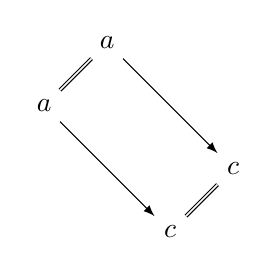
\begin{tikzpicture}[>=latex,baseline,scale=0.8]
   \node (a) at (2,2) {$a$};
   \node (b) at (1,1) {$a$};
   \node (c) at (4,0) {$c$};
   \node (d) at (3,-1) {$c$};

   \draw [double] (a) -- (b) ;
   \draw [->] (a) -- (c) ;
   \draw[->] (b) -> (d) ;
   \draw[double] (c) -> (d) ;
\end{tikzpicture} 
% one reduction
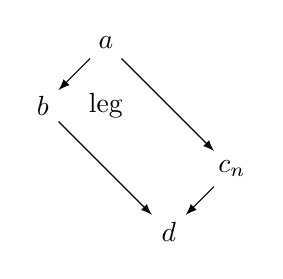
\begin{tikzpicture}[>=latex,baseline,scale=0.8]
   \node (a) at (2,2) {$a$};
   \node (b) at (1,1) {$b$};
   \node (cn) at (4,0) {$c_n$};
   \node (dn) at (3,-1) {$d$};
   \node (ih) at (2,1) {leg};

   \draw [->] (a) -- (b) ;
   \draw [->] (a) -- (cn) ;
   \draw[->] (b) -> (dn) ;
   \draw[->] (cn) -> (dn) ;
\end{tikzpicture} 
% more steps in both sides
\begin{tikzpicture}[>=latex,baseline,scale=0.8]
   \node (a) at (2,2) {$a$};
   \node (b1) at (1,1) {$b_1$};
   \node (c1) at (3,1) {$c_1$};
   \node (bn) at (-1,-1) {$b_n$};
   \node (cn) at (5,-1) {$c_n$};
   \node (d1) at (0,-2) {$d_1$};
   \node (dn) at (2,-4) {$d_n$};
   \node (leg) at (1,0) {leg} ;
   \node (ih) at (3,-1) {i.h.};

   \draw [->] (a) -- (b1) ;
   \draw [->] (a) -- (c1) ;
   \draw [->] (b1) -- (bn) ;
   \draw [->] (c1) -- (cn) ;
   \draw[->] (c1) -> (d1) ;
   \draw[->] (bn) -> (d1) ;
   \draw[->] (d1) -> (dn) ;
   \draw[->] (cn) -> (dn) ;
\end{tikzpicture}
\end{proof}

\begingroup\par\noindent\advance\leftskip\mathindent\(
\begin{pboxed}\SaveRestoreHook
\column{B}{@{}>{\hspre}l<{\hspost}@{}}%
\column{3}{@{}>{\hspre}l<{\hspost}@{}}%
\column{5}{@{}>{\hspre}l<{\hspost}@{}}%
\column{24}{@{}>{\hspre}l<{\hspost}@{}}%
\column{37}{@{}>{\hspre}l<{\hspost}@{}}%
\column{57}{@{}>{\hspre}l<{\hspost}@{}}%
\column{58}{@{}>{\hspre}l<{\hspost}@{}}%
\column{59}{@{}>{\hspre}l<{\hspost}@{}}%
\column{E}{@{}>{\hspre}l<{\hspost}@{}}%
\>[3]{}\Varid{diamond-cr-steps}\;\mathbin{:}\;\{\mskip1.5mu \Varid{⟿}\;\mathbin{:}\;\Conid{Rel}\mskip1.5mu\}\;\Varid{→}\;\Varid{diamond}\;\Varid{⟿}\;\Varid{→}\;\Varid{cr-steps}\;\Varid{⟿}{}\<[E]%
\\
\>[3]{}\Varid{diamond-cr-steps}\;\Varid{♢}\;\{\mskip1.5mu \Varid{a}\mskip1.5mu\}\;\{\mskip1.5mu \Varid{.a}\mskip1.5mu\}\;\{\mskip1.5mu \Varid{c}\mskip1.5mu\}\;{}\<[37]%
\>[37]{}\Varid{zero}\;{}\<[59]%
\>[59]{}\Varid{a⟿*c}\;{}\<[E]%
\\
\>[3]{}\hsindent{2}{}\<[5]%
\>[5]{}\mathrel{=}\;\Varid{c},\Varid{a⟿*c},\Varid{zero}{}\<[E]%
\\
\>[3]{}\Varid{diamond-cr-steps}\;\Varid{♢}\;{}\<[37]%
\>[37]{}(\Varid{one}\;\Varid{a⟿b})\;{}\<[58]%
\>[58]{}\Varid{a⟿*c}{}\<[E]%
\\
\>[3]{}\hsindent{2}{}\<[5]%
\>[5]{}\mathbf{with}\;\Varid{leg}\;\Varid{♢}\;\Varid{a⟿b}\;\Varid{a⟿*c}{}\<[E]%
\\
\>[3]{}\Varid{...}\;\mid \;\Varid{d},\Varid{b⟿*d},\Varid{c⟿d}\;\mathrel{=}\;\Varid{d},\Varid{b⟿*d},\Varid{one}\;\Varid{c⟿d}{}\<[E]%
\\
\>[3]{}\Varid{diamond-cr-steps}\;\Varid{♢}\;\{\mskip1.5mu \Varid{a}\mskip1.5mu\}\;\{\mskip1.5mu \Varid{bₙ}\mskip1.5mu\}\;\{\mskip1.5mu \Varid{.a}\mskip1.5mu\}\;{}\<[37]%
\>[37]{}(\Varid{more}\;\Varid{a⟿b₁}\;\Varid{b₁⟿*bₙ})\;{}\<[57]%
\>[57]{}\Varid{zero}\;{}\<[E]%
\\
\>[3]{}\hsindent{2}{}\<[5]%
\>[5]{}\mathrel{=}\;\Varid{bₙ},\Varid{zero},\Varid{more}\;\Varid{a⟿b₁}\;\Varid{b₁⟿*bₙ}{}\<[E]%
\\
\>[3]{}\Varid{diamond-cr-steps}\;\Varid{♢}\;{}\<[37]%
\>[37]{}(\Varid{more}\;\Varid{a⟿b₁}\;\Varid{b₁⟿*bₙ})\;{}\<[57]%
\>[57]{}(\Varid{one}\;\Varid{a⟿c}){}\<[E]%
\\
\>[3]{}\hsindent{2}{}\<[5]%
\>[5]{}\mathbf{with}\;\Varid{leg}\;\Varid{♢}\;\Varid{a⟿c}\;(\Varid{more}\;\Varid{a⟿b₁}\;\Varid{b₁⟿*bₙ}){}\<[E]%
\\
\>[3]{}\Varid{...}\;\mid \;\Varid{d},\Varid{c⟿*d},\Varid{bₙ⟿d}\;\mathrel{=}\;\Varid{d},\Varid{one}\;\Varid{bₙ⟿d},\Varid{c⟿*d}{}\<[E]%
\\
\>[3]{}\Varid{diamond-cr-steps}\;\Varid{♢}\;{}\<[37]%
\>[37]{}(\Varid{more}\;\Varid{a⟿b₁}\;\Varid{b₁⟿*bₙ})\;{}\<[57]%
\>[57]{}(\Varid{more}\;\Varid{a⟿c₁}\;\Varid{c₁⟿*cₙ}){}\<[E]%
\\
\>[3]{}\hsindent{2}{}\<[5]%
\>[5]{}\mathbf{with}\;\Varid{leg}\;\Varid{♢}\;\Varid{a⟿c₁}\;(\Varid{more}\;\Varid{a⟿b₁}\;\Varid{b₁⟿*bₙ}){}\<[E]%
\\
\>[3]{}\Varid{...}\;\mid \;\Varid{d₁},\Varid{c₁⟿*d₁},\Varid{bₙ⟿d₁}{}\<[E]%
\\
\>[3]{}\hsindent{2}{}\<[5]%
\>[5]{}\mathbf{with}\;\Varid{diamond-cr-steps}\;\Varid{♢}\;\Varid{c₁⟿*d₁}\;\Varid{c₁⟿*cₙ}{}\<[E]%
\\
\>[3]{}\Varid{...}\;\mid \;\Varid{dₙ},\Varid{d₁⟿*dₙ},\Varid{cₙ⟿*dₙ}{}\<[E]%
\\
\>[3]{}\hsindent{2}{}\<[5]%
\>[5]{}\mathrel{=}\;\Varid{dₙ},\Varid{more}\;\Varid{bₙ⟿d₁}\;{}\<[24]%
\>[24]{}\Varid{d₁⟿*dₙ},\Varid{cₙ⟿*dₙ}{}\<[E]%
\ColumnHook
\end{pboxed}
\)\par\noindent\endgroup\resethooks

Since both statements of the transitive closure are equivalent,
from cr-steps we can deduce church-rosser for any relation having
the diamond property.

\begingroup\par\noindent\advance\leftskip\mathindent\(
\begin{pboxed}\SaveRestoreHook
\column{B}{@{}>{\hspre}l<{\hspost}@{}}%
\column{3}{@{}>{\hspre}l<{\hspost}@{}}%
\column{E}{@{}>{\hspre}l<{\hspost}@{}}%
\>[3]{}\Varid{diamond-cr}\;\mathbin{:}\;\{\mskip1.5mu \Varid{⟿}\;\mathbin{:}\;\Conid{Rel}\mskip1.5mu\}\;\Varid{→}\;\Varid{diamond}\;\Varid{⟿}\;\Varid{→}\;\Varid{cr}\;\Varid{⟿}{}\<[E]%
\\
\>[3]{}\Varid{diamond-cr}\;\Varid{♢}\;\mathrel{=}\;\Varid{cr-steps-to-cr}\;(\Varid{diamond-cr-steps}\;\Varid{♢}){}\<[E]%
\ColumnHook
\end{pboxed}
\)\par\noindent\endgroup\resethooks

\begin{lemma} 
Let $R$ and $S$ be two relations such that $S\subseteq R$ and $\transclos R\subseteq S$, if
$R$ is Church-Rosser, then $S$ is also.
\end{lemma}
\begin{proof}
The proof is immediate: let $a\,\transclos S\,b$ and $a\,\transclos S\,c$, by the first hypothesis and $mon-star$\ lemma
we know both $a\,\transclos R\,b$ and $a\,\transclos R\,c$. By Church-Rosser for $R$ we get an element
$d$ with proofs of $b\,\transclos R\,d$ and $c\,\transclos R\,d$; by the second hypothesis and $trans-⊆-star$\ lemma we conclude
$b\,\transclos S\,d$ and $c\,\transclos S\,d$.
\end{proof}

\begingroup\par\noindent\advance\leftskip\mathindent\(
\begin{pboxed}\SaveRestoreHook
\column{B}{@{}>{\hspre}l<{\hspost}@{}}%
\column{3}{@{}>{\hspre}l<{\hspost}@{}}%
\column{5}{@{}>{\hspre}l<{\hspost}@{}}%
\column{8}{@{}>{\hspre}l<{\hspost}@{}}%
\column{32}{@{}>{\hspre}c<{\hspost}@{}}%
\column{32E}{@{}l@{}}%
\column{E}{@{}>{\hspre}l<{\hspost}@{}}%
\>[3]{}\Varid{cr-⊆}\;\mathbin{:}\;\{\mskip1.5mu \Conid{R}\;\Conid{S}\;\mathbin{:}\;\Conid{Rel}\mskip1.5mu\}\;\Varid{→}\;\Conid{S}\;\Varid{⊆}\;\Conid{R}\;\Varid{→}\;\Conid{R}\;\Varid{⊆}\;\Varid{star}\;\Conid{S}\;\Varid{→}\;\Varid{cr}\;\Conid{R}\;\Varid{→}\;\Varid{cr}\;\Conid{S}{}\<[E]%
\\
\>[3]{}\Varid{cr-⊆}\;\Conid{S⊆R}\;\Conid{R⊆S⋆}\;\Varid{cr}\;\Varid{aR⋆b}\;\Varid{aR⋆c}{}\<[E]%
\\
\>[3]{}\hsindent{2}{}\<[5]%
\>[5]{}\mathbf{with}\;\Varid{cr}\;(\Varid{mon-star}\;\Conid{S⊆R}\;\Varid{aR⋆b})\;(\Varid{mon-star}\;\Conid{S⊆R}\;\Varid{aR⋆c}){}\<[E]%
\\
\>[3]{}\Varid{...}\;\mid \;\Varid{d},\Varid{bR⋆d},\Varid{cR⋆d}{}\<[E]%
\\
\>[3]{}\hsindent{2}{}\<[5]%
\>[5]{}\mathrel{=}\;{}\<[8]%
\>[8]{}\Varid{d}{}\<[32]%
\>[32]{},{}\<[32E]%
\\
\>[8]{}\Varid{trans-⊆-star}\;\Conid{R⊆S⋆}\;\Varid{bR⋆d}{}\<[32]%
\>[32]{},{}\<[32E]%
\\
\>[8]{}\Varid{trans-⊆-star}\;\Conid{R⊆S⋆}\;\Varid{cR⋆d}{}\<[E]%
\ColumnHook
\end{pboxed}
\)\par\noindent\endgroup\resethooks
%</Relation>

\end{document}


%\printbibliography


